\documentclass{classrep}
\usepackage[utf8]{inputenc}
\frenchspacing

\usepackage{graphicx}
\usepackage[usenames,dvipsnames]{color}
\usepackage[hidelinks]{hyperref}
\usepackage{lmodern}
\usepackage{placeins}
\usepackage{amsmath, amssymb, mathtools}
\usepackage{listings}
\usepackage{fancyhdr, lastpage}

\pagestyle{fancyplain}
\fancyhf{}
\renewcommand{\headrulewidth}{0pt}
\cfoot{\thepage\ / \pageref*{LastPage}}

%--------------------------------------------------------------------------------------%
\studycycle{Informatyka stosowana, studia dzienne, II st.}
\coursesemester{I}

\coursename{Wprowadzenie do Data Science i metod uczenia maszynowego}
\courseyear{2020/2021}

\courseteacher{mgr inż. Rafał Woźniak}
\coursegroup{Wtorek, 13:15}

\author{%
    \studentinfo[239673@edu.p.lodz.pl]{Michał Kidawa}{239673}
}

\title{Zadanie 1.: Problem Set 1}

\begin{document}
    \maketitle
    \thispagestyle{fancyplain}

    \section{Wprowadzenie}
    \label{intro} {
        Żyjemy w czasach powszechnej i niezwykle łatwej wymiany informacji. Bardzo często natrafimy na statystyki, które działają na nas opiniotwórczo w ramach określonej dziedziny. Podczas analizy wniosków płynących z danych statystyk warto mieć na uwadze ich źródło oraz czynniki związane z doborem próby. Wpływają one znacznie na uzyskane wyniki i na pierwszy rzut oka są trudne do wykrycia. Zły wybór próby jest niezwykle rozległym tematem. Poniższa analiza problemu obejmuje zagadnienia związane z doborem próby nieodzwierciedlającym rzeczywistego stanu populacji, dobór za małej próby, który prowadzi do uzyskania ekstremalnych wyników oraz wpływ czynnika ludzkiego podczas gromadzenia danych do analizy próby statystycznej.
    }

    \section{Przykłady błędnego doboru próby do analizy statystycznej}
    \label{wrong_examples} {

        \subsection{Próba, które nieodzwierciedla rzeczywistości}
        \label{wrong_examples:reality} {
            Ciekawy przykład doboru próby, która nieodzwierciedlała rzeczywistości można było zaobserwować podczas wyborów prezydenckich w Stanach Zjednoczonych w 1936 roku. Popularny magazyn \emph{Literary Digest} przeprowadził sondę wśród potencjalnych wyborców, która miała wskazać który z kandydatów (Alfred Langdon, czy Franklin D. Roosevelt) zostanie następnym prezydentem Stanów zjednoczonych. Łącznie zebrano dane od około 2.4 miliona osób, co stanowiło gigantyczną liczbę badanych. Były to osoby posiadające telefon i subskrybenci magazynu, które zgodziły się na wzięcie udziału w badaniu. Uczestnicy sondy wskazali Langdona jako następnego prezydenta z przewagą 57\% do 43\% Roosevelt'a. Wynik okazał się zupełnie odwrotny (62\% Roosevelt - 38\% Langdon) Może się wydawać, że taka próba była miarodajna. \emph{Literaly Digest} popełniło jednak błąd w doborze osób biorących udział w badaniu. Analizując profil przeciętnego ankietowanego widzimy, że jest to osoba posiadająca telefon lub subskrypcję magazynu. Można zatem wnioskować, iż była przedstawicielem klasy średniej lub wyższej. W 1936 roku telefon definitywnie był produktem, na który mogła pozwolić sobie znaczna mniejszość społeczeństwa \cite{digest_study}. Tego typu błąd nazywany jest \emph{błędem wyboru}. Oznacza to, że wybór osób, grup lub danych do analizy został przeprowadzony w sposób, który nie zapewnił właściwej randomizacji, powodując w ten sposób, że uzyskana próbka nie jest reprezentatywna dla populacji.
        }

        \subsection{Małe próby prowadzą do niepoprawnych wyników}
        \label{wrong_examples:small-sample} {
            Przykłady doboru zbyt małej próby mają miejsce m.in. w branży medycznej i farmakologicznej. Załóżmy, że dokonujemy analizy porównawczą 2 grup badanych, której celem jest określenie częstotliwości występowania powikłań po zastosowaniu terapii. Wykazano, że po określonej terapii w leczeniu że częstotliwość występowania powikłań po zastosowaniu terapii lekiem X wynosi 0.1\% co zostało udowodnione w badaniach eksperymentalnych fazy przedklikinczej. Jeżeli zdefiniujemy grupę pacjentów liczącą 100-200 osób możliwe, że dojdzie do sytuacji w której dane powikłanie może nie wystąpić, co nie znaczy, że dany preparat nie powoduje powikłań. Należy w takim przypadku pamiętać o mocy testu, która jest zależna od wielkości próby użytej w badaniu. Zakładając, że dane zostały wybrane w sposób poprawny większa próba będzie lepiej obrazowała populację. Ponadto w przypadku wybrania mniej licznej próby istnieje szansa, że będą to jednostki wyjątkowe. Problem doboru za małej próby jest ściśle związany z problematyką opisaną w sekcji \ref{wrong_examples:reality}. Jeśli liczność próby jest zbyt mała to od razu stanowi niepoprawną reprezentację faktycznej populacji. Załóżmy, że wykonujemy 5 rzutów monetą. Istnieje szansa, że 80\% tych rzutów zakończy się "wylosowaniem" tej samej strony. Nie jest to jednak w żaden sposób miarodajna próba i nie zgadza się ona z zasadami prawdopodobieństwa.
            
            \begin{figure}[!htbp]
                \centering
                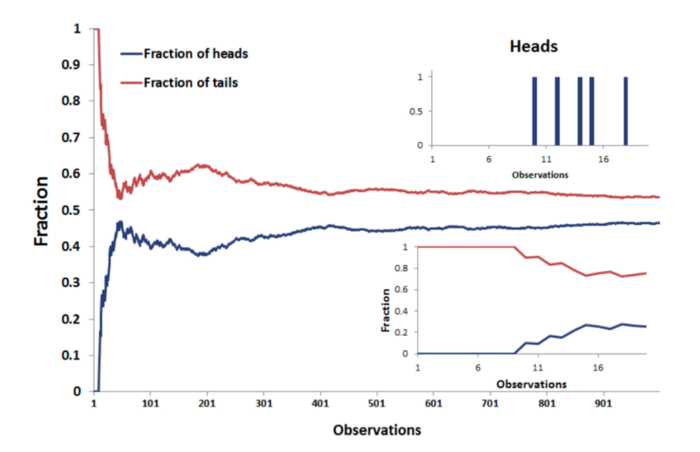
\includegraphics
                [width=0.8\textwidth,keepaspectratio]
                {img/heads.png}
                \caption
                [Wykres prezentujący wyniki rzutu monetą]
                {Wykres prezentujący wyniki rzutu monetą; można zauważyć, że mała liczba prób powoduje ekstremalne wyniki \cite{towardsdatascience_article}}
                \label{heads}
            \end{figure}
            \FloatBarrier
        }

        \subsection{Czynnik ludzki przy zbieraniu danych}
        \label{wrong_examples:social-des} {
            Istnieją tematy, w przypadku których respondenci mają skłonność do udzielania nieprawdziwych odpowiedzi, aby zaprezentować się w możliwie jak najlepszym świetle. Efekt ten nazwany jest \textit{Efektem społecznych oczekiwań} (ang. social desirability bias). Jest to jeden z najczęściej występujących źródeł błędów, które pływają na wyniki badań ankietowych. Uwydatnia się on szczególnie w przypadku drażliwych społecznie kwestii takich jak religia, polityka czy sprawy osobiste, takie używki lub higiena. Jeśli zadalibyśmy napotkanym na ulicy Polakom pytanie, jak często biorą prysznic uzyskane dane najpewniej byłyby obarczone błędem wynikającej z opisanego powyżej efektu. Ankietowani zawyżaliby celowo liczbę swoich kąpieli ponieważ brak zachowania higieny jest działaniem niepożądanym w społeczeństwie.   
        }
    }

    \section{Rozwiązanie problemów}
    \label{good_examples} {
        Aby zapobiegać \textit{błędowi wyboru} należy wykorzystywać metody wybory podgrupy z populacji, które zapewniają jak największą losowość. Jest to możliwe oczywiście do pełnego stopnia, a do tego wykorzystanie odpowiednich metod doboru wiąże się ze zwiększonymi kosztami przeprowadzenia badań. Ponadto warto upewnić się, że wybrana próba jak najlepiej odzwierciedla faktyczny rozkład cech kluczowych względem całej populacji.
    
        Jeśli chodzi o rozmiar próby nie ma jednoznacznego wzoru, który potrafi określić, jaka konkretnie liczność będzie odpowiednia przy danej populacji. Dzięki większej próbie jesteśmy w stanie osiągnąć lepszą moc testu, czyli prawdopodobieństwo niepopełnienia błędu drugiego rzędu.
    
        W celu zwalczania \textit{efektu społecznych oczekiwań} wyróżniono metody, które mają na celu zmniejszenie jego wpływu na wynik badania takie jak użycie testu wymuszonego wyboru, technika losowych odpowiedzi, czy też technika pozornego wariografu \cite{coping}.  
    }

    \section{Wnioski} {
        Po analizie tematu można dość do wniosku, że: 
        \begin{itemize}
            \item przed przyswojeniem i wzięciem za pewnik informacji prezentowanej w postaci statystyk warto poznać metodę zbierania danych
            \item dobór populacji ma istotny wpływ na wynik prowadzonych badań / eksperymentu
            \item statystyki mogą być łatwo użyte w celu manipulacji odbiorcą
        \end{itemize}
    }

    \begin{thebibliography}{0}
        \bibitem
        {digest_study}
        {https://www2.math.upenn.edu/~deturck/m170/wk4/lecture/case1.html}
        \bibitem
        {towardsdatascience_article}
        {https://towardsdatascience.com/lessons-from-how-to-lie-with-statistics-57060c0d2f19}
        \bibitem{coping}
        {Nederhof AJ. Methods of coping with social desirability bias: A review. „European Journal of Social Psychology”. 15 (3), s. 263–80, 1985}
    \end{thebibliography}

\end{document}
